\section{Design af spoler}\label{sec:sec_spole_design}
\emph{Introduktion til emnet i kapitlet skrives her}
For at kunne dimensionere og designe en spole, er det væsentligt at vide hvilket formål spolen skal bruges til. Spolen har mange egenskaber, og i dette projekt vil de blive designet, så de kan bruges som sensorer. Altså en enhed der opfanger eller udsender et analogt signal. 

Som beskrevet tidligere, består systemet af i alt 3 spoler. 1 stor spole, som skal stå for at udsende et signal. Herudover 2 mindre identiske spoler, som skal opfange signalerne. For et illustrativt billede af opsætningen se afsnit **.
\husk{Simon}{Indsæt afsnitsnummer}

I den følgende tekst, vil der blive beskrevet hvilke faktorer der er blevet lagt vægt på, samt hvordan nogle af Maxwells ligninger er blevet brugt til at dimensionere de enkelte spoler. Herunder begreber som magnetfelt(B), flux$(\Phi)$, induktans(L) og elektromotorisk kraft som fremadrettet vil blive betegnet som EMF$(\xi)$. 

Først vil dimensioneringen af den store spole tages højde for, hvorefter der kigges på de 2 små spoler.
Den færdige dimensionering skal ende ud i et målbart EMF signal.

Der er som udgangspunkt taget brug af Biot-Savarts lov som ses i ligning \ref{eq:spole_biot_savart}, 
\subsection{Magnetfelt}
\husk{Kenneth}{Til Simon: Større bogstaver på tegning.}
\begin{figure}[h!]
	\centering
	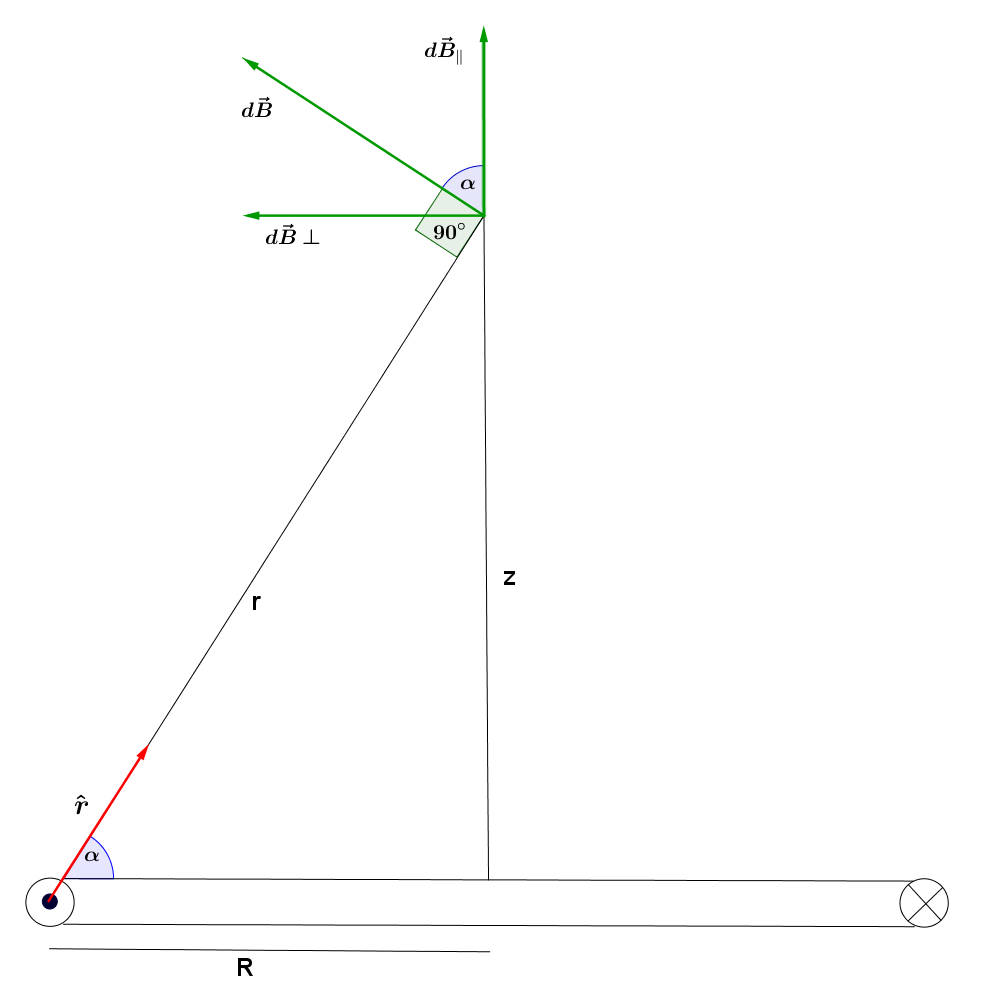
\includegraphics[width=.6\textwidth]{billeder/B_felt.png}
	\caption{Cirkulær leder med radius R}
	\label{fig:spole_fig1}
\end{figure}

På figur \ref{fig:spole_fig1} ses et tværsnit af en cirkulær leder, hvori der løber en strøm kaldet $i$. Krydset indikerer at stømmen går ind i papiret, og prikken også kaldet spidsen af en pil, indikerer at strømmen går ud af papiret. Man kan også se på denne figur, som den store spole med 1 vinding. Betragt punktet P på z aksen. I dette punkt ønskes et magnetfelts styrke bestemt, afhængig af positionen z. Som det ses er vinklen, uanset hvor på lederen man befinder sig, mellem $d\vec{s}$ og enhedsvektoren $\hat{r}$ altid $90\degree$ vinkeltret på hinanden.

Med dette kan $d\vec{B}$ feltet tegnes ind, vha. Biot-Savarts lov, eller vha. højrehåndreglen. En mere overskuelig måde at se det på er, at krydsproduktet af 2 vektorer, er en vektor der står vinkeltret på begge. 
$d\vec{B}$ kan nu deles op i 2 komposanter. En komposant $dB_\parallel$, som står parralelt på z axen og den cirkulære leder. Derudover også en komposant $dB_\perp$, som står vinkeltret på samme.

Summen af alle de vinkeltrette komposanter går ud da $d\vec{s}\times d\vec{B}_\perp=0$, og tilbage står kun de parallelle komposanter $dB_\parallel$, hvilket resulterer i:

 \begin{align}
 &B=\int dB_\parallel \label{eq:B_field}
 \end{align}

  
  
Betragt Biot-Savarts lov i ligning \ref{eq:spole_biot_savart}

\begin{align}
&d\vec{B}=\frac{\mu_0}{4\pi} \frac{i d\vec{s} \times \hat{r}}{r^2}\label{eq:spole_biot_savart}
\end{align}

Fra figur \ref{fig:spole_fig1}, kan ligning \ref{eq:spole_biot_savart} skrives om til:
\begin{align}
&dB=\frac{\mu_0}{4\pi} \frac{i ds\: sin(90\degree)}{r^2}\label{eq:spole_biot_savart2}
\end{align}
 Denne ligning giver udtryk for hvad det magnetiske felt er i en afstand $r$ fra $d\vec{s}$.
 
Ud fra figur \ref{fig:spole_fig1}, kan et udtryk for $dB_\parallel$ også vises.

 \begin{align}
 	&dB_\parallel=dB\: cos(\alpha)
 \end{align}

Hermed kan et samlet udtryk for $dB_\parallel$ gives: 

\begin{align}
&dB_\parallel=\frac{\mu_0 \:i\: cos(\alpha)\:ds}{4\:\pi\: r^2}
\end{align}

Da det er z der ønskes varieret, bliver et nyt udtryk nødt til at blive bestemt, hvor z indgår. Betragt figur \ref{fig:spole_fig1} igen. Her ses, at $r$ og vinklen $\alpha$, er relateret til hinanden, og ved hjælp at Phytagoras, kan disse 2 udtryk findes:


\begin{align}
&r=\sqrt{R^2+z^2}
\end{align}

og

\begin{align}
&cos(\alpha)=\frac{R}{r}=\frac{R}{\sqrt{R^2+z^2}}
\end{align}

Da $i, R$ og $z$ alle har samme værdi for alle $ds$ hele vejen rundt i den cirklære leder, kan man vha. integration summere op, på samme måde som deffineret i ligning \ref{eq:B_field}, og der fås dermed et udtryk for B:



\begin{align}
&B=\frac{\mu_0 \: i \: R}{4\pi(R^2+z^2)^\frac{3}{2}}\int ds
\end{align}

Grænseværdierne for $\int ds$ er den cirkulære leders omkreds.

\begin{align}
&\int\limits_{0}^{2\pi R} ds = 2\pi R
\end{align}

Et endeligt udtryk for magnetfeltet $B(z)$ gives i ligning \ref{eq:Bz_field}.

\begin{align}
	&B(z)=\frac{\mu_0 \: i \: R^2}{2(R^2+z^2)^\frac{3}{2}} \label{eq:Bz_field}
\end{align}


Da dette udtryk kun er gældende for en cirkulær leder, altså en spole med 1 vinding, skal et nyt udtryk bestemmes. Dette udtryk tager udgangspunkt i ligning \ref{eq:Bz_field}, som blev udledt før.

\begin{figure}[h!]
	\centering
	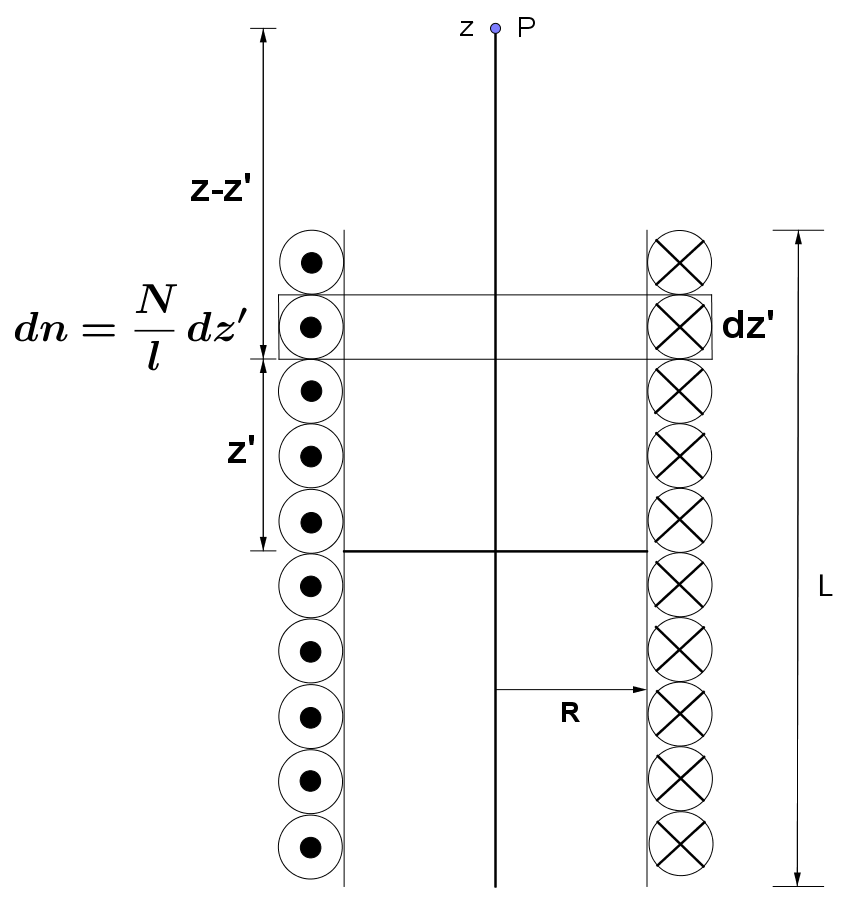
\includegraphics[width=.5\textwidth]{billeder/B_felt2.png}
	\caption{Solenoid med radius R}
	\label{fig:spole_fig2}
\end{figure}

Formlen for B feltet i en uendelig lang solenoid er givet ved:

\begin{align}
	&B=\mu ni
\end{align}

Hvor $n$ er antal vindinger pr. længde:


\begin{align}
	&n=\frac{N}{L}
\end{align}

I dette udtryk er B feltet centreret i midten af den uendelig lange solenoide.

Da solenoidestørrelsen er bestemt, og ikke uendelig lang, samt $B$ feltet ligger uden for solenoidens yderkant, skal en ny ligning af $B$ feltet bestemmes.
Det antages at $B$ feltet er homogent omkring hele fladen, og ikke kun i det punkt der bestemmes.


Betragt figur \ref{fig:spole_fig2}. Her ses tværsnittet af en solenoide, med z aksen i centrum. Det ønskede $B$ felt skal bestemmes i punktet $P$.

Det ses at størrelsen af $dn$ er proportional med tykkelsen $dz'$:

\begin{align}
	&dn=\frac{N}{L} dz'
\end{align}



Ud fra ligning \ref{eq:Bz_field}, kan $dB(z)$ udtrykkes ved: 

\begin{align}
	&dB(z)=\frac{\mu_0 \: i \: R^2}{2(R^2+(z-z')^2)^\frac{3}{2}}dn=\frac{\mu_0 \: N \: i \: R^2}{2L(R^2+(z-z')^2)^\frac{3}{2}}dz'
\end{align}

Ved at integrerer over hele længden på solenoiden fås:

\begin{align}
	&B(z)=\int\limits_{-\frac{L}{2}}^{\frac{L}{2}}\frac{\mu_0 \: N \: i \: R^2}{2L(R^2+(z-z')^2)^\frac{3}{2}}dz'
\end{align}

Og et endeligt udtryk:
\begin{align}
	&B(z)= \frac{\mu_0 \: i \: R^2 \: N}{2L}\left(\frac{\frac{L}{2}-z}{\sqrt{(z-\frac{L}{2})^2+R^2}}+\frac{\frac{L}{2}+z}{\sqrt{(z+\frac{L}{2})^2+R^2}}\right)
\end{align}

\subsection{Flux og elektromotorisk kraft}
I dette afsnit vil den magnetiske flux blive bestemt.  
Faraday lavede et eksperiment, og fandt ud af, at et magnetfelt der ændrer sig over tid i en lukket lederkreds, skabte en induceret EMF inde i kredsen.
Dette lavede han et udtryk for:

\begin{align}
	&EMF(\xi) = - \frac{d\Phi}{dt}
\end{align}

Denne lov er også kendt for navnet Lenz's lov, da han kom frem til det omvendte fortegn.

Flux i den lille spole hidrørende fra den store spole, ved fuld overlappelse er bestemt ved:

\begin{align}
	&\Phi_{21} = BA_2
\end{align}

Hvor $B$ er det magnetiske felt, og $A_2$ er arealet på den lille spoles overflade.
Da $B$ feltet er homogent på hele overfladen, antages $B$ konstant. 

Ud fra dette udtryk, kan den totale EMF, der er induceret over i den lille spole blive bestemt ved følgende udtryk:

\begin{align}
	&\xi = -N_2\frac{d\Phi_{21}}{dt} \label{eq:emf_lille_spole}
\end{align}

Hvor $N_2$ er antal vindinger i den lille spole.
\\ \\
Det er ikke nødvendigt at beregne den store spoles flux, i og med selvinduktansen kendes og dermed kan spændingen i den store spole findes ved:

\begin{align}
	&V = L\frac{di}{dt} \label{eq:ldidt}
\end{align}

\subsection{Strømfortrængning}\label{Sec_skineff.}
I forbindelse med valg af trådtykkelse på kobbertråden, som skal vikles rundt om spolerne, er strømfortrængningen i ledningen væsentlig.\\
Hvis signalet i spolerne havde været et rent DC signal, kunne strømmen antages homogent i hele tværsnitsarealet i kobbertråden.
Da dette ikke er tilfældet, vil AC signalet "fotrænge" ud i kanten af koppertrådens tværsnitsareal. 
Der bliver derved skabt et hulrum inden i koppertråden. \\
Herved bliver modstanden i kobbertråden ændret.
AC modstanden i koppertråden findes ved ligning \ref{eq:R_AC}.

\begin{align}
	& R_{AC}=\frac{\rho l}{A_{eff}} \label{eq:R_AC}
\end{align}
Hvor
\begin{align}
	& \rho = \text{Resistiviteten i koppertråden} \nonumber
\end{align}
\begin{align}
	& l = \text{Længden af koppertråden} \nonumber
\end{align}
\begin{align}
	& A_{eff} = \text{Det effektive areal af strømfortrængningen = $\delta\pi\times\cdot diameter$} \nonumber
\end{align}
	
Frekvensen i spolerne, er dimensioneret forholdsvis høje, hvilket vil betyde strømfortrængning.  \\
Formlen for strømfortrænging er givet ved ligning \ref{eq:skineffect}.
\begin{align}
	& \delta = \sqrt{\frac{\rho}{\pi f\mu_0\mu_r}} \label{eq:skineffect}
\end{align}

Hvor 



\begin{align}
	& f = \text{Frekvensen} \nonumber
\end{align}

\begin{align}
	& \mu_0 = \text{Permabilitetskonstant som er givet ved $4\pi 10^{-7}\henry/\meter$} \nonumber
\end{align}

\begin{align}
	& \mu_r = \text{Den relative permabilitetskonstant for kopper} \nonumber
\end{align}
\husk{Simon}{indsæt link som reference: http://chemandy.com/calculators/round-wire-ac-resistance-calculator.htm 5/12-16. kl 13}


\subsection{Resultater}
I følgende afsnit er den teoretiske del blevet anvendt, til at finde de værdier, der bliver brugt i spoledesignet.\\
Derudover, vil målinger foretaget med et oscilloskop blive analyseret og teorien eftervist.\\ 
Tykkelsen på kobbertråden, vælges meget tynd af flere grunde.
Én af grundene, er pga. plads, men som udangspunkt dimensioneret ud fra afsnit \ref{Sec_skineff.}. \\
Der ønskes en så lav modstand som muligt.  
Dette gælder både for den store, og de små spoler.\\
Med hensyn til det fysiske design af spolehuset, henvises til afsnit\husk{Simon}{Indsæt henvisning}
Et fuldstændigt overblik over alle værdier for spolerne, som er dimensioneret ud fra teorien, findes herunder.
\begin{align}
&i=0.05\cdot \sin{(2pi\cdot 46936\cdot t)} \nonumber
\end{align}
\begin{align}
&\mu_0 =4\pi 10^{-7}T\cdot \m/A \nonumber
\end{align}
\begin{align}
&l = 0.01\m \nonumber
\end{align}
\begin{align}
&\text{Trådtykkelse} = 0.25\mm \nonumber
\end{align}
\begin{align}
&N_1=63\nonumber
\end{align}
\begin{align}
&N_2=300\nonumber
\end{align}
\begin{align}
&R_1=0.0175\m\nonumber
\end{align}
\begin{align}
&R_2=0.00855\m\nonumber
\end{align}
\begin{align}
&A_1=9.6211\cdot 10^{-4} \m^2\nonumber
\end{align}
\begin{align}
&A_2=2.2966\cdot 10^{-4} \m^2\nonumber
\end{align}

\subsubsection{Stor spole}

Den store spole er bestemt ud fra, at den skal fungere som en enhed, der skal sende et signal videre. 
Signalet i denne, skal derfor være forholdsvis kraftigt, dermed også B feltet.
\begin{figure}[h!]
	\centering
	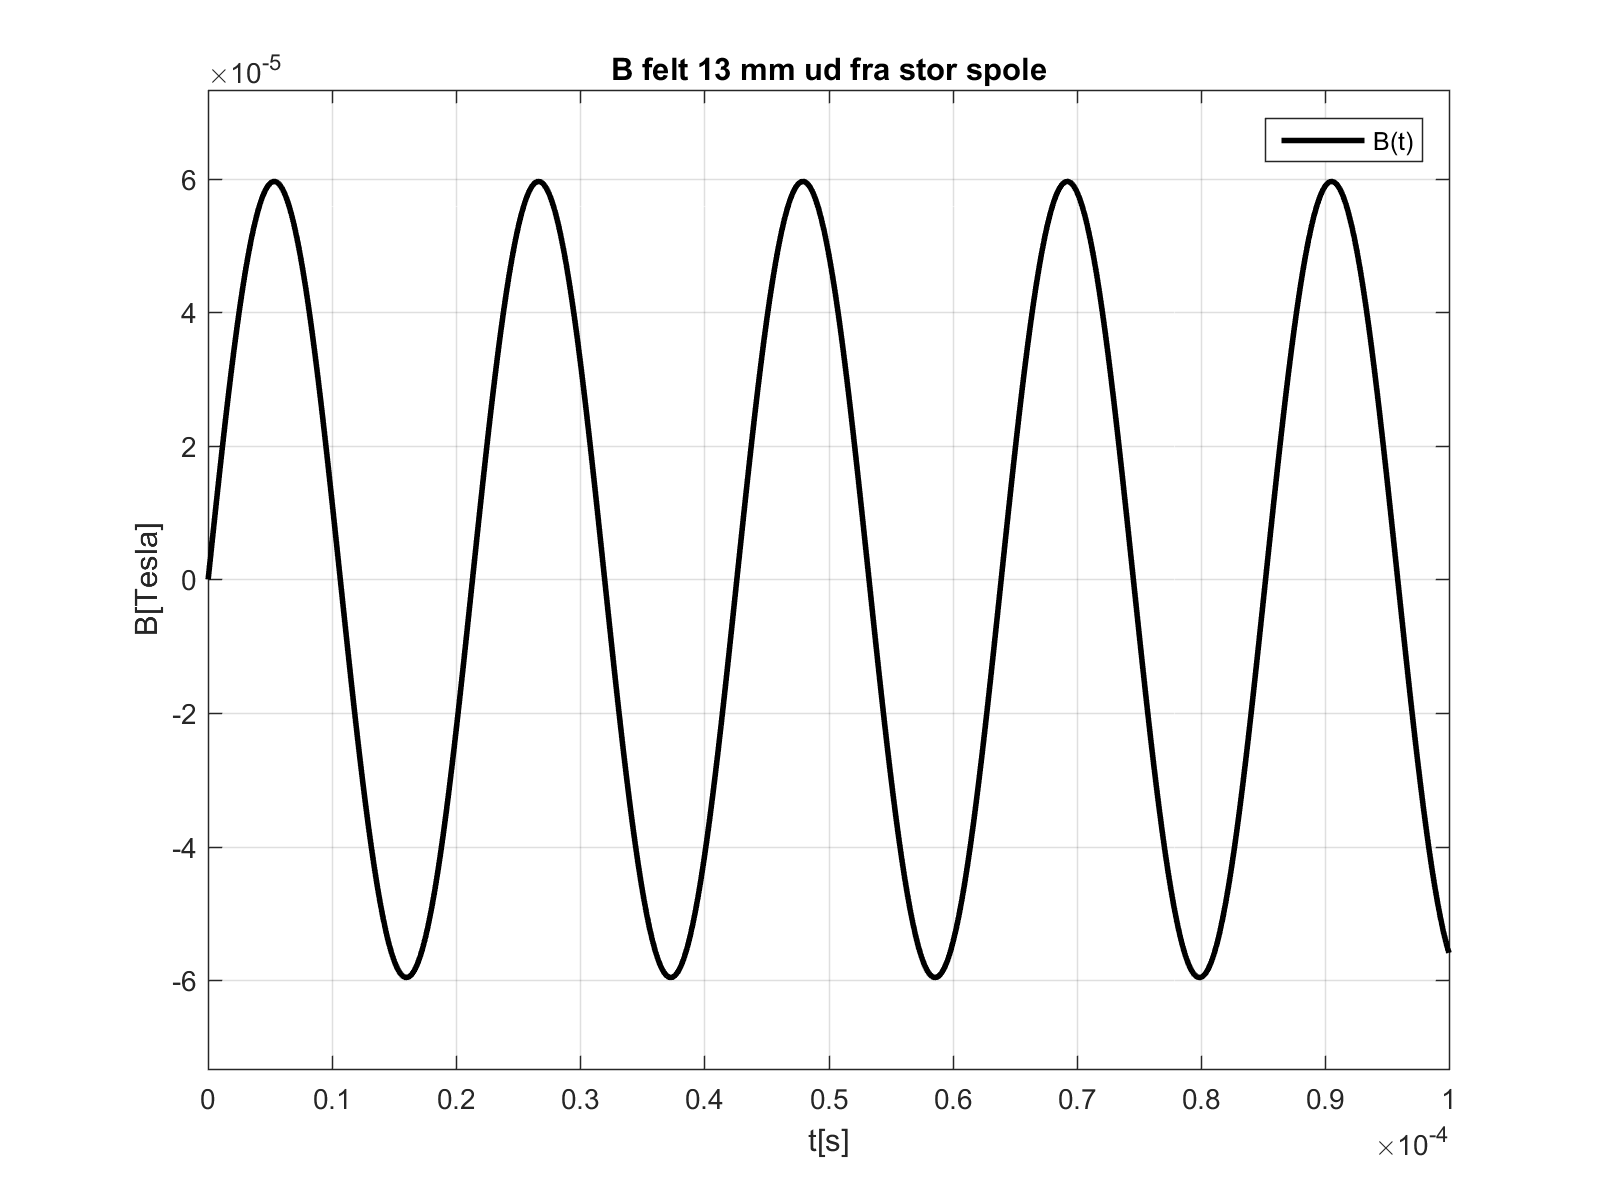
\includegraphics[width=.3\textwidth]{billeder/B_felt_stor_spole.png}
	\caption{Magnetfeltet beregnet 13 $\mm$ ud fra stor spole}
	\label{fig:B_felt_stor_spole}
\end{figure}

\begin{figure}[h!]
	\centering
	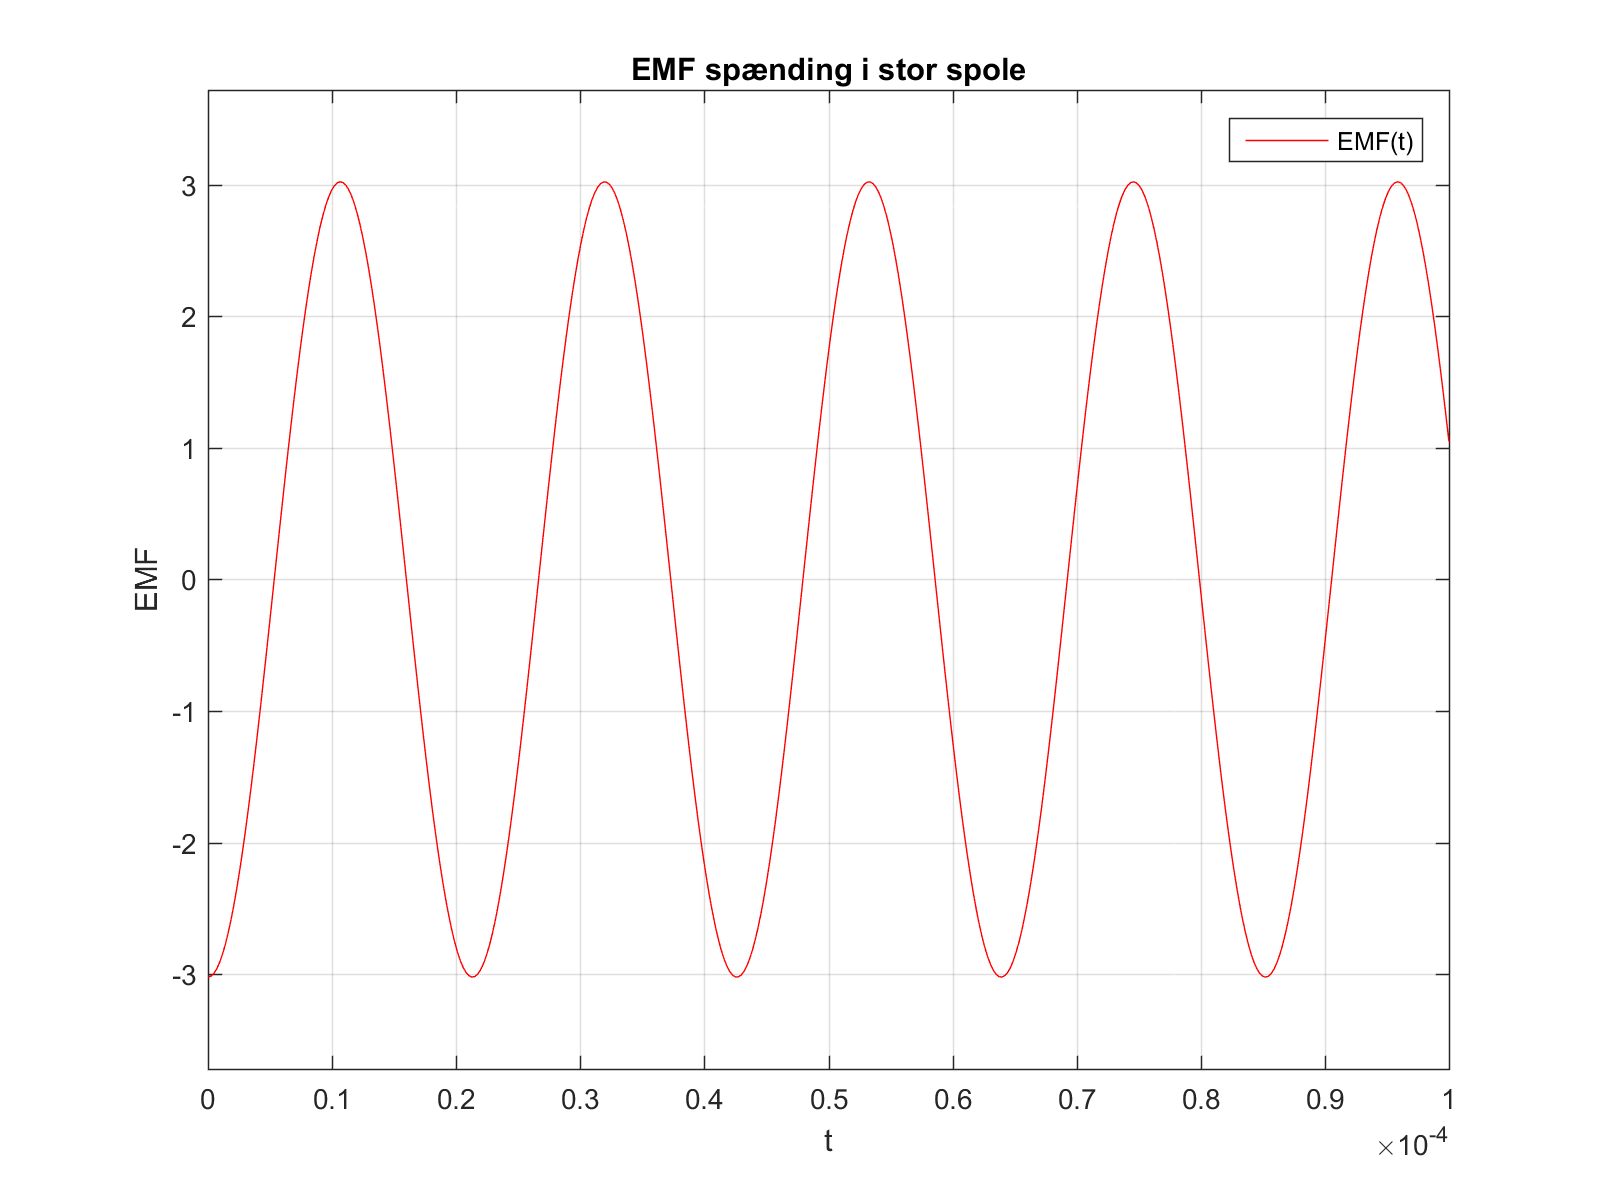
\includegraphics[width=.3\textwidth]{billeder/EMF_stor_spole.png}
	\caption{EMF spænding i stor spole}
	\label{fig:EMF_stor_spole}
\end{figure}
I figur \ref{fig:EMF_stor_spole}, ses en graf der viser spænding som funktion af tiden i den store spole. se ligning \ref{eq:ldidt}, hvor $i$ er givet ved: 

\begin{align}
&i=0.05\cdot \sin{(2pi\cdot 46936\cdot t)}
\end{align}
Frekvensen og peakstrømmen er dimensioneret ud fra afsnit \ref{sec:Frev_gen} \\
Her ses en induceret spænding med en peak to peak på ca. 6\volt.
\subsubsection{Lille spole}
\begin{figure}[h!]
	\centering
	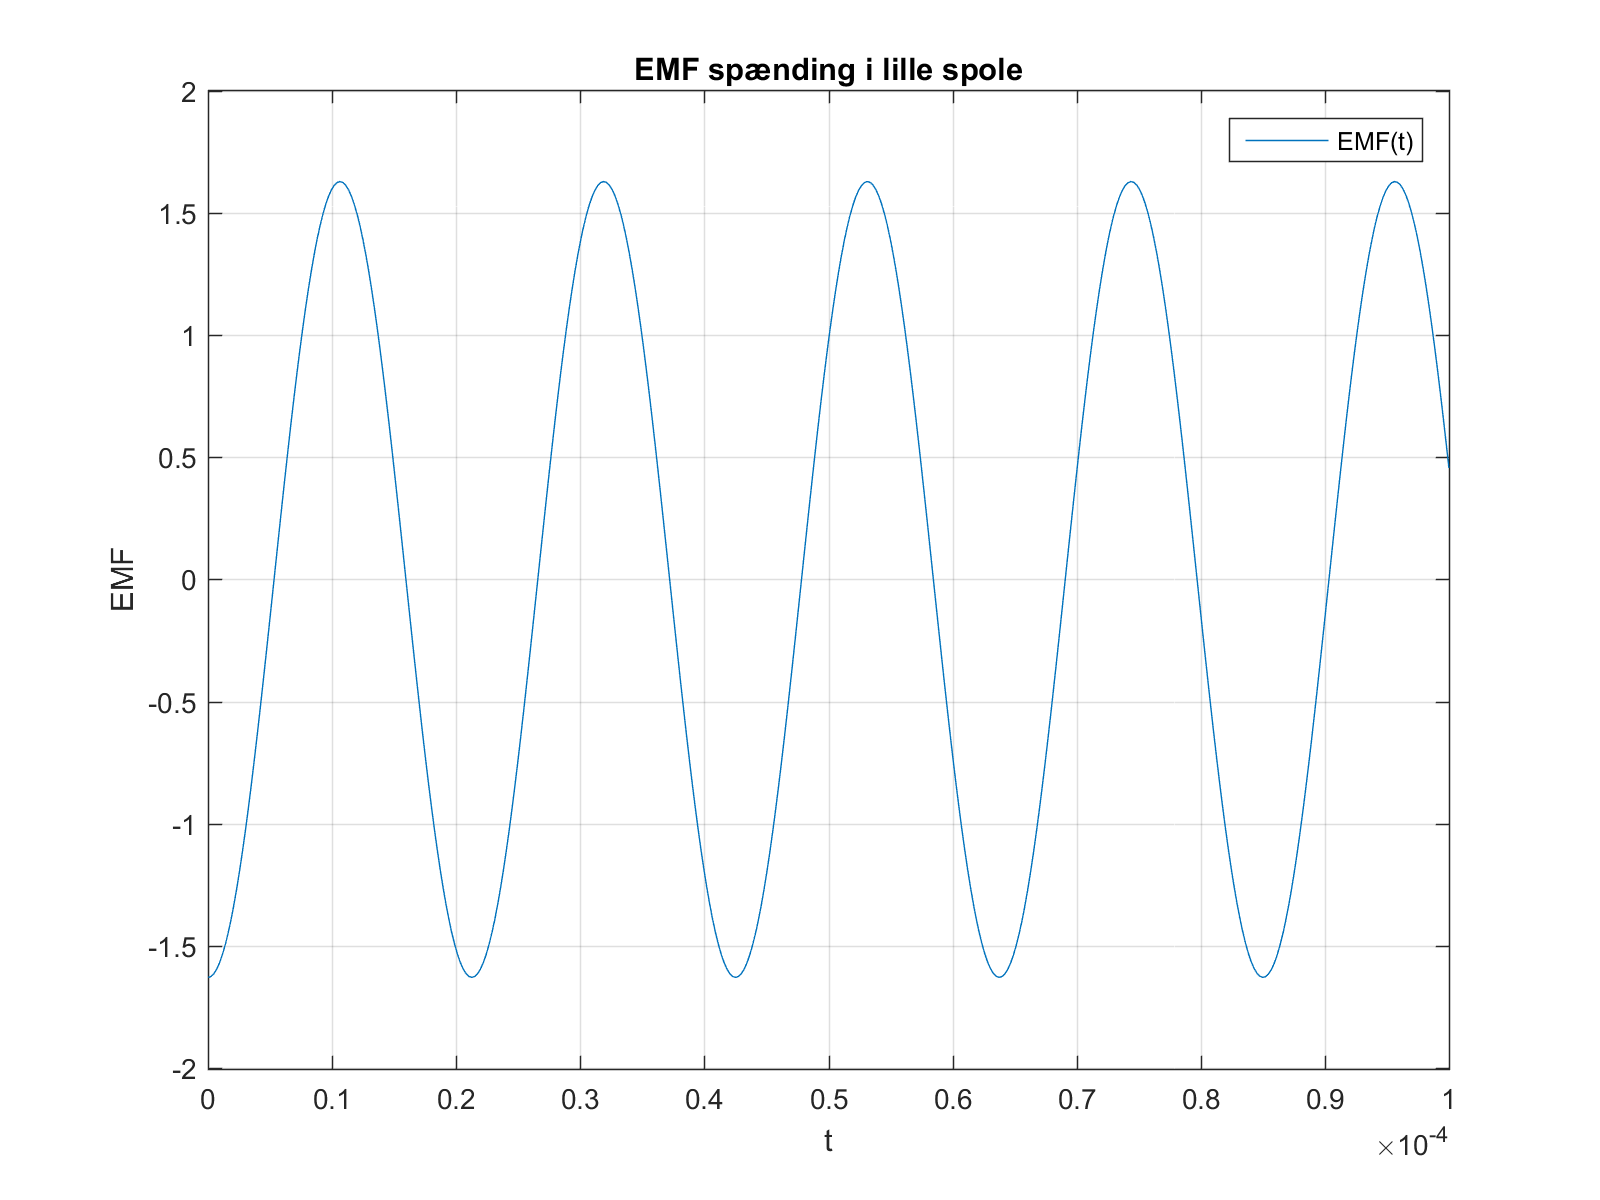
\includegraphics[width=.6\textwidth]{billeder/EMF_lille_spole.png}
	\caption{EMF spænding i lille spole}
	\label{fig:EMF_lille_spole}
\end{figure}





\husk{Simon}{Juster billeder}



 






\subsection{3D design/fysisk design af spolehus}
For at kunne gøre disse spoler til en realitet, er der lavet specialdesignede spolehuse som passer perfekt til de udregnede værdier. Disse spoler er blevet tegnet i 3D-CAD programmet Inventor, og derefter 3D-printet på en 3D-printer. \\

Spolerne er designet således at når den store spole er i nul (i midten) overlapper den de mindre spoler så de er dækket præcist 50\percent. Når den store spole så er i sin fulde udslagsvinkel er hhv. den ene mindre spole dækket helt, hvor den anden slet ikke er dækket. \\

\husk{fraannk}{Overvej om dette er overflødigt}

Disse spoler er designet med brugervenlighed i bagtankerne. For at vi ikke skal designe et nyt spolehus for hver gang vi vikler en ny spole, er der lavet et Plug-n-play system hvor kan nemt kan "klikke" nye spoler i. Dette er lige så meget for at undgå spild af filament. Derudover er der lavet huller, så det er nemt at putte dem i vindingsmaskinen. \\

Da basen af køretøjet er noget der er taget fra et tidligere projekt, er spolerne lavet sådan, at de nemt er til at klikke på det nuværende pendul, samt køretøjets bundplade. \\

\husk{fraannk}{Indsæt billæj}

Derudover er der designet en batteriholder samt printmonteringsplade som også udnytter de nuværende huller i bilens bundplade. 

\begin {itemize}
\item Udnytter forudborede huller
\item Batteri"slots"
\item Standoff mounts til print
\end {itemize}